\subsection{Congruence Experimentation}\label{experimentation}
To create the classifier, the efficacy of individual approaches needs to be evaluated. The general structure of each experiment run takes the following form:

\begin{enumerate}
	\item Implement the classifier approach under test
	\item Compile and load the dataset according to the parameters discussed in section \ref{experimentation-data}
	\item Run the algorithm on each article in the dataset, measuring the resultant classification
	\item Record the accuracy of the classifier using the dataset as a baseline truth
	\item Calculate the significance	values of the outcome, and optionally plot a chart to represent the results, if appropriate
\end{enumerate}

\subsubsection{Experimentation Dataset}\label{experimentation-data}
At the time of experimentation, the bespoke labelled dataset was not yet complete, as not enough ratings had been given to calculate an average rating per article. In lieu of this, the FNC-1 dataset was used as a gold standard against which to measure the preliminary experiments. The dataset contains articles labelled as \texttt{agree}, \texttt{disagree}, \texttt{discuss}, or \texttt{unrelated}. Articles labelled as \texttt{discuss} were discarded from the set before experimentation - if an article discusses the content, it could ultimately either agree or disagree with the headline, so it provides no meaningful information considering the scope of this project. Articles tagged as \texttt{unrelated} were also discarded, as they comprised of body texts matched with headlines from a different article, which will not be present in the articles collected. Once the FNC-1 dataset was cleaned, 843 labelled articles remained.


\subsubsection{Sentiment Analysis}
The VADER sentiment analyser\footnote{\url{https://github.com/cjhutto/vaderSentiment}} was used for experimentation - it would not be the best use of time to design a bespoke analyser if no trend was discovered in the dataset. The code used to perform this experiment is displayed in appendix \ref{app:sentiment-analysis}.


\begin{figure}
	\centering
	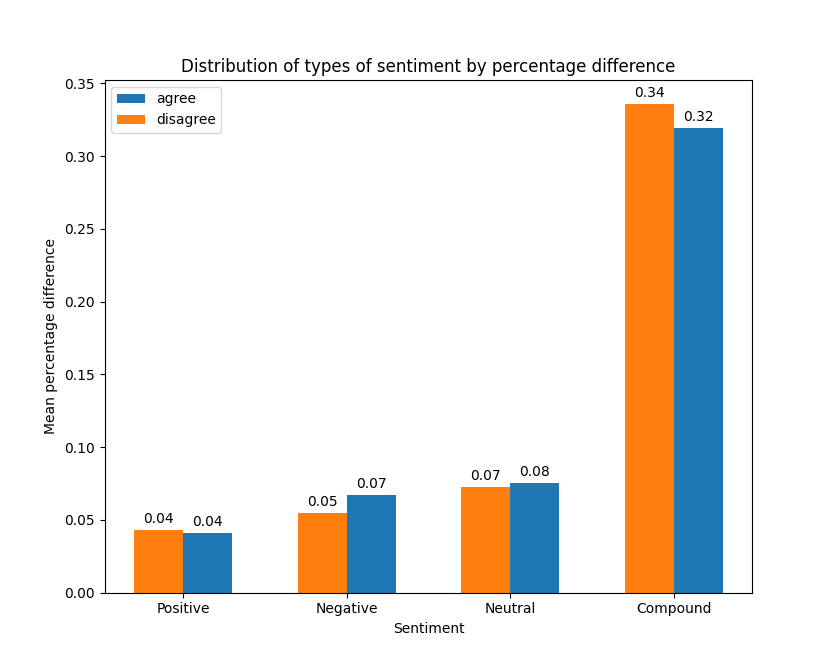
\includegraphics[width=0.8\linewidth]{images/plots/sentiment-analysis.png}
	\caption{Distribution of sentiment types in the FNC-1 dataset}\label{plot:sentiment-analysis}
\end{figure}

\vspace{5mm}

\hspace{-6mm}\begin{minipage}{0.65\linewidth}
VADER produces 3 measures of sentiment - negativity, positivity and neutrality - as well as a compound value of all of them. To visualise the dataset, the percentage difference of the headline and the body text's measures was plotted. The results are shown in figure \ref{plot:sentiment-analysis}. Table \ref{tab:sentiment-sig} shows the results of a significance test; the data had a non-Guassian distribution so a Mann-Whitney U test was used.\\
\end{minipage}
\hspace{5mm}
\begin{minipage}{0.3\linewidth}
\vspace{-12mm}
\begin{tabular}{ll}
\textbf{Sentiment} & \textbf{p-value} \\
Positive           & 0.20988          \\
Negative           & 0.0667           \\
Neutral            & 0.37534          \\
Compound           & 0.08266         
\end{tabular}
\captionof{table}{Sentiment\\analysis significance}
\label{tab:sentiment-sig}
\end{minipage}


No clear trend in the difference between articles that agree and disagree is visible in the plot. Additionally, as none of the p-values is below 0.05, the results lack significance and must be rejected. This quite strongly shows there is no correlation between the difference in the sentiment of headlines and articles, and as a result, sentiment analysis will not provide a meaningful use in the creation of the classifier.

This result is not surprising - the difference between sentiment and congruence was covered in section \ref{lit:sentiment-analysis}. It is possible for two pieces of text to have different sentiments and be in concurrence, or to have similar sentiments and be opposed in meaning, which means sentiment analysis is not suited for this approach.

\subsubsection{Word Vectorisation}
Another approach tested was word vectorisation - codifying a token as a vector comprised of numbers representing a certain quality of the word's meaning, using the context windows discussed in section \ref{lit:word2vec}.

Gensim's Python implementation of word2vec\footnote{\url{https://radimrehurek.com/gensim/models/word2vec.html}} was trained on articles from the raw dataset. As the training data is only used to give word2vec an understanding of how words relate to each other and not used to determine congruence, the data does not need to be labelled. Ten iterations of learning and 250,000 articles were used to train a model with 300 nodes.

The vectorisation model created is of good quality, and able to perform mathematical operations on words, such as the often-used example:

\[\textrm{Woman} + \textrm{King} - \textrm{Man} = \textrm{Queen}\]

With the model trained, it can be used to evaluate the labelled FNC dataset.
For each article in the database, an average vector was calculated for both the headline and the body. This was achieved by summing up each word's vector and dividing by the number of words in the text. The similarity of these vectors was then computed using the \texttt{cosine\_similarites} function in Gensim, which calculates the cosine difference of two vectors. The average difference for both articles that agree and disagree was obtained. The code used to perform this experiment is displayed in appendix \ref{app:vectorisation}.

For articles labelled as agree, the average vector difference was 0.5175, and those labelled disagree had a difference of 0.5050, with a p-value of 0.19308. Like with the sentiment analysis experiment, the lack of significance and the negligible difference between each average shows that this is an ineffective way to determine congruence. This could be because only a few of the words in an article will point to incongruence - by obtaining an average of all of them, the text's meaning will be lost in the noise.

\subsubsection{tf-idf}

\begin{minipage}{0.65\linewidth}
To ascertain the practicality of using tf-idf to detect incongruence, the algorithm set out in section \ref{lit:tfidf} was implemented in Python. To get an informal understanding of the implementation's efficacy, it was used to determine the relevance of a range of keywords to an article about a house fire caused by fireworks. The results are shown in table \ref{tab:tfidf-terms}. As the table shows, the implementation is working as expected - more relevant words, such as 'ablaze', have higher tf-idf values, indicating a higher relevance, and terms such as 'and' and 'football' have a much lower, negligible value.
\\
\end{minipage}
\hspace{5mm}
\begin{minipage}{0.3\linewidth}
\vspace{-2mm}
\begin{tabular}{ll}
\textbf{Term} & \textbf{tf-idf value} \\
ablaze & 421.500 \\
fireworks & 168.600 \\
explosive & 93.667 \\
the & 0.089 \\
and & 0.058 \\
football & 0.000
\end{tabular}
\captionof{table}{tf-idf values for a range of terms}
\label{tab:tfidf-terms}
\end{minipage}

To apply the algorithm to the problem, tf-idf was used to calculate each word's relevance in an article's headline to its body text. A mean was then taken of those values, as shown below. A full code listing is available in the Github repository.\footnote{\url{https://github.com/jacobbarrow/honours/tree/master/experiments/tfidf.py}}

\begin{lstlisting}[language=Python]
for article in articles.values():
    tfidfs = []
    for word in article['headline']:
        tfidfs.append(tfidf(word, article['body'], domain))

    mean = numpy.mean(tfidfs)
\end{lstlisting}

The mean will give an overall relevance between the headline and body of an article. The means were classified according to the article's labelled stance (agree/disagree) and then analysed. For articles labelled as agree, the average tf-idf mean of their headlines was 0.1167. For those labelled disagree, the average was 0.0718. While this difference may initially seem promising, with a p-value of 0.26281, the results must be rejected.

This result is disappointing but expected; tf-idf is used to determine the relevance of a word to a document and does not account for the document's overall sentiment. For instance, consider the following two statements:

\begin{itemize}
	\item Mauve is a trendy colour to paint a house
	\item The worst colour to paint a house is mauve
\end{itemize}

The term 'mauve' appears the same number of times for both of them, so according to tf-idf will have identical relevance. However, each statement's sentiments are opposed, something unable to be determined by just the relevance alone. 

Additionally, using the mean of all headline values may be 'muddying the waters' of the relevancy, as happened in the word vectorisation experiment. However, this may not be as strong a factor, as the difference between a relevant word and an irrelevant word is large, as seen in table \ref{tab:tfidf-terms}, and so would have a more significant effect on the mean.